\documentclass[11pt,aspectratio=169]{beamer}
\usetheme{Madrid}
\usecolortheme{default}

\usepackage[utf8]{inputenc}
\usepackage{amsmath, amssymb}
\usepackage{graphicx}
\usepackage{booktabs}
\usepackage{hyperref}
\usepackage{caption}
\captionsetup{font=scriptsize,labelfont=scriptsize}

\graphicspath{{../report/figures/}}

\title[Pairs Trading Strategy]{Pairs Trading Strategy Framework \\ \large with Risk Controls}
\subtitle{MA8.402: Mathematics for Finance}
\author[Raghava, Hruday, Trivedi, Agarwal]{Nijesh Raghava \and Vivek Hruday \and Kushagra Trivedi \and Tanishq Agarwal}
\date{Spring '26}

\begin{document}

\begin{frame}
    \titlepage
\end{frame}

\begin{frame}{Outline}
    \tableofcontents
\end{frame}

\section{Introduction}
\begin{frame}{Introduction to Pairs Trading}
    \begin{itemize}
        \item \textbf{Statistical Arbitrage}: Exploiting short-term market microstructure noise, liquidity shocks, or transient behavioral biases.
        \vspace{0.2cm}
        \item \textbf{Pairs Trading Premise}: Two assets with similar fundamental drivers will maintain a stable long-term relationship.
        \vspace{0.2cm}
        \item \textbf{Mechanism}: Short the outperforming asset and buy the underperforming one when prices diverge, expecting mean reversion.
        \vspace{0.2cm}
        \item \textbf{Our Core Hypothesis}: Incorporating \textbf{Granger causality} into the selection pipeline significantly enhances out-of-sample robustness and risk-adjusted returns over traditional Pearson correlation.
    \end{itemize}
\end{frame}

\section{Mathematical Foundations}
\begin{frame}{Stochastic Processes \& Cointegration}
    \begin{itemize}
        \item \textbf{Asset Prices}: Modeled as Geometric Brownian Motion (GBM). Individual log-prices $p_{i,t}$ are non-stationary $I(1)$ processes.
        \item \textbf{Cointegration}: Two $I(1)$ series are cointegrated if a linear combination results in a stationary $I(0)$ series.
        \begin{equation*}
            S_t = p_{y,t} - \beta p_{x,t}
        \end{equation*}
        \item \textbf{Engle-Granger Two-Step Method}:
        \begin{enumerate}
            \item Estimate cointegrating regression using OLS: $p_{y,t} = \alpha + \beta p_{x,t} + \epsilon_t$
            \item Test residuals for stationarity using Augmented Dickey-Fuller (ADF) test.
        \end{enumerate}
    \end{itemize}
\end{frame}

\begin{frame}{Modeling the Spread: Ornstein-Uhlenbeck Process}
    \begin{itemize}
        \item A stationary spread $S_t$ can be mathematically modeled using the continuous-time \textbf{Ornstein-Uhlenbeck (OU)} process:
        \begin{equation*}
            dS_t = \theta (\mu - S_t) dt + \sigma dW_t
        \end{equation*}
        \begin{itemize}
            \item $\mu$: long-term equilibrium mean
            \item $\theta > 0$: speed of mean reversion
            \item $\sigma$: volatility of the spread
        \end{itemize}
        \vspace{0.2cm}
        \item \textbf{Half-life of Mean Reversion}: Expected time for the spread to halve its deviation from the mean:
        \begin{equation*}
            \tau = \frac{\ln(2)}{\theta}
        \end{equation*}
    \end{itemize}
\end{frame}

\begin{frame}{Causality vs. Correlation}
    \begin{itemize}
        \item \textbf{Correlation Fallacy}: Pearson correlation simply measures the degree to which two variables move together. Correlation does not imply cointegration or causation (spurious regressions).
        \vspace{0.3cm}
        \item \textbf{Granger Causality}: Time series $X$ Granger-causes $Y$ if past values of $X$ help predict $Y$ beyond past values of $Y$ alone.
        \item We use \textbf{Vector Autoregression (VAR)} and require strong bi-directional or uni-directional Granger causality (p-value $< 0.05$).
        \item \textbf{Result}: Filters out spurious correlations driven by exogenous market factors.
    \end{itemize}
\end{frame}

\section{Signal Generation \& Risk Management}
\begin{frame}{Dynamic Signals \& Position Sizing}
    \begin{itemize}
        \item \textbf{Dynamic Z-Score}: Based on rolling mean ($\mu_{S,t}$) and volatility ($\sigma_{S,t}$).
        \begin{equation*}
            Z_t = \frac{S_t - \mu_{S,t}}{\sigma_{S,t}}
        \end{equation*}
        Trade entry when $|Z_t| \geq Z_{\text{entry}}$, exit when $|Z_t| \leq Z_{\text{exit}}$.
        \vspace{0.3cm}
        \item \textbf{Inverse Volatility Sizing}:
        Maintains a constant gross exposure risk profile. Size is scaled inversely to the recent volatility of spread changes.
        \begin{equation*}
            k_t = \frac{E_{\text{target}}}{\max(\sigma_{\Delta S, t}, \sigma_{\text{min}})}
        \end{equation*}
    \end{itemize}
\end{frame}

\begin{frame}{Risk Management Engine}
    Strict capital preservation measures are enforced via overlays:
    \vspace{0.3cm}
    \begin{itemize}
        \item \textbf{Stop Loss}: Active positions liquidated instantly if cumulative PnL drops below a predefined fraction of allocated capital (e.g., -5\%).
        \vspace{0.2cm}
        \item \textbf{Time Stop}: Given theoretical half-life $\tau$, positions held longer than $T_{\text{max}}$ (e.g., 30 days) are flattened (mean-reverting relationship breakdown).
        \vspace{0.2cm}
        \item \textbf{Value at Risk (VaR)}: Rolling 95\% historical VaR is monitored to ensure the portfolio's tail risk remains within institutional bounds.
    \end{itemize}
\end{frame}

\section{Software Architecture}
\begin{frame}{System Architecture Overview}
    Our modular, object-oriented framework consists of 5 decoupled engines:
    \vspace{0.2cm}
    \begin{enumerate}
        \item \textbf{\texttt{DataDownloader}}: yfinance API ingestion with \texttt{joblib} local filesystem caching for rapid backtesting.
        \item \textbf{\texttt{PairIdentificationEngine}}: $\mathcal{O}(N^2)$ pairwise correlation matrix, Engle-Granger coint tests, and VAR Granger causality tests.
        \item \textbf{\texttt{PairSignalEngine}}: Calculates rolling Z-scores and generates normalized dollar weights via inverse-volatility scaling, capping absolute exposure.
        \item \textbf{\texttt{PairRiskEngine}}: Intercepts raw signals to enforce Stop Loss, Time Stop, and VaR overlays before execution.
        \item \textbf{\texttt{PairBacktestEngine}}: The accounting ledger. Simulates daily mark-to-market, exact transaction costs (turnover), and computes net PnL/Sharpe.
    \end{enumerate}
\end{frame}

\section{Experimental Results \& Visual Analysis}
\begin{frame}{Experimental Setup \& Initial Results}
    \begin{itemize}
        \item \textbf{Universe}: 20 liquid U.S. large-cap equities.
        \item \textbf{In-Sample}: Jan 2020 -- Dec 2022.
        \item \textbf{Out-of-Sample}: Jan 2023 -- Jan 2024.
    \end{itemize}
    \vspace{0.2cm}
    \begin{table}
        \centering
        \caption{Out-of-Sample Performance Summary}
        \begin{tabular}{@{}lccc@{}}
            \toprule
            \textbf{Approach} & \textbf{Total Net PnL (\$)} & \textbf{Max Drawdown} & \textbf{Sharpe Ratio} \\
            \midrule
            Correlation & -5,706.35 & -7.80\% & -0.738 \\
            Causal & \textbf{4,275.69} & \textbf{-5.74\%} & \textbf{0.516} \\
            \bottomrule
        \end{tabular}
    \end{table}
    The causal approach achieved a positive Sharpe ratio, whereas correlation pairs suffered a severe out-of-sample breakdown.
\end{frame}

\begin{frame}{Performance \& Drawdown Analysis}
    \begin{columns}
        \begin{column}{0.5\textwidth}
            \centering
            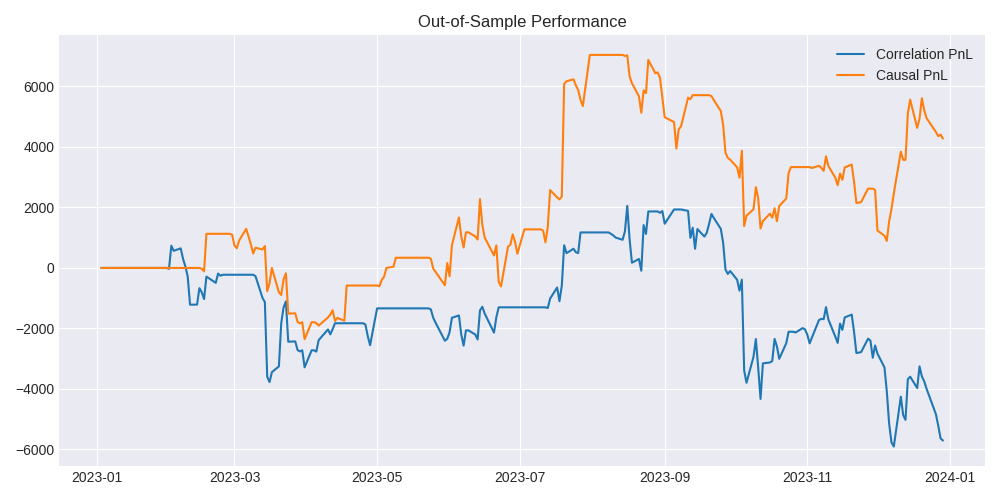
\includegraphics[width=\textwidth,height=0.55\textheight,keepaspectratio]{viz1_performance.png}
            \vspace{0.1cm}
            \scriptsize \\ \textbf{Insight 1}: Causal PnL climbs steadily. Correlation PnL drops massively halfway through 2023 due to exogenous shocks.
        \end{column}
        \begin{column}{0.5\textwidth}
            \centering
            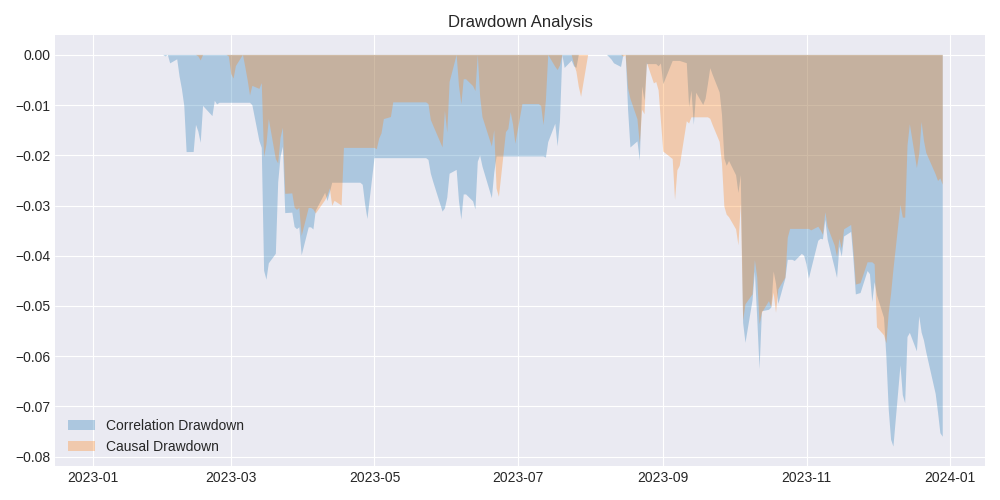
\includegraphics[width=\textwidth,height=0.55\textheight,keepaspectratio]{viz2_drawdown.png}
            \vspace{0.1cm}
            \scriptsize \\ \textbf{Insight 2}: Correlation spends most of OOS in deep drawdown. Causal experiences milder, short-lived drawdowns.
        \end{column}
    \end{columns}
\end{frame}

\begin{frame}{Return Distribution \& Causality Verification}
    \begin{columns}
        \begin{column}{0.5\textwidth}
            \centering
            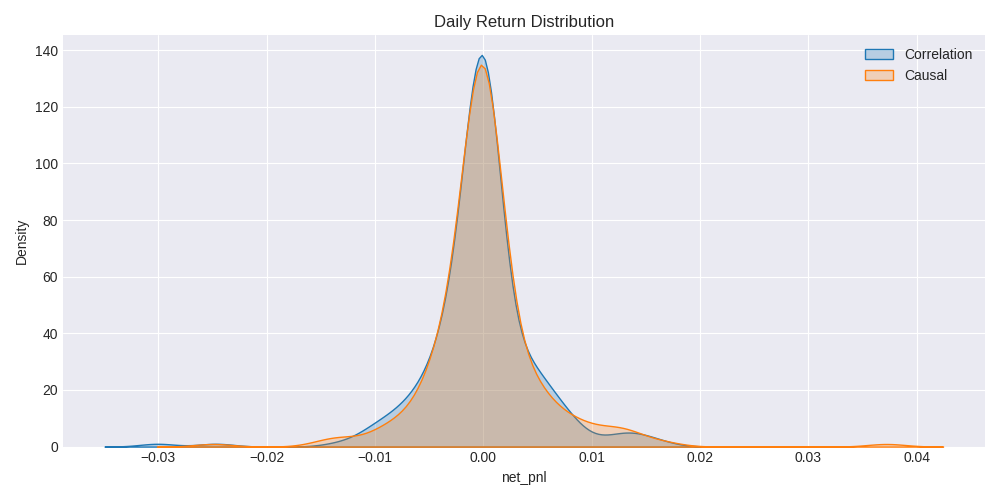
\includegraphics[width=\textwidth,height=0.55\textheight,keepaspectratio]{viz3_returns_kde.png}
            \vspace{0.1cm}
            \scriptsize \\ \textbf{Insight 3}: Causal returns have a tighter distribution shifted right (consistent gains). Correlation is left-skewed (frequent large losses).
        \end{column}
        \begin{column}{0.5\textwidth}
            \centering
            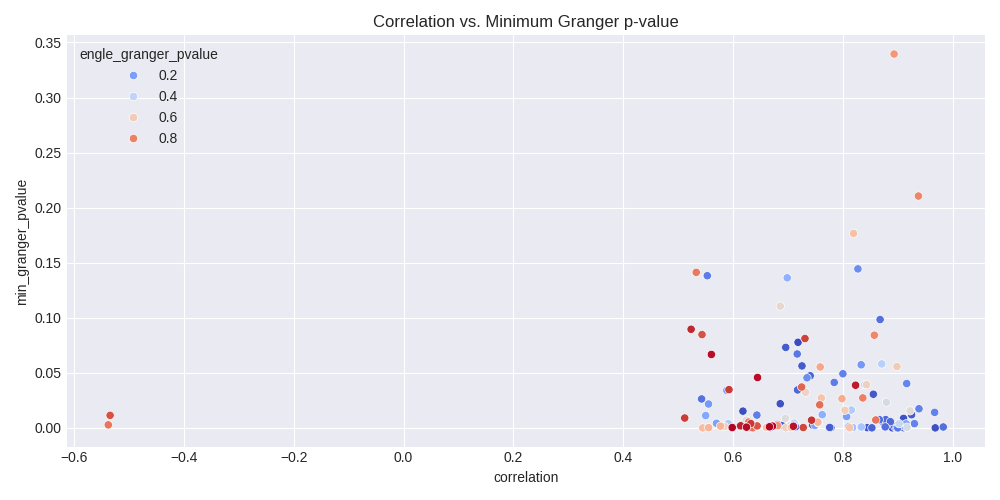
\includegraphics[width=\textwidth,height=0.55\textheight,keepaspectratio]{viz7_corr_vs_causal.png}
            \vspace{0.1cm}
            \scriptsize \\ \textbf{Insight 7}: High correlation does NOT guarantee low Granger p-value. Superior pairs exist in the bottom-right quadrant.
        \end{column}
    \end{columns}
\end{frame}

\begin{frame}{Sensitivity: Transaction Costs \& Stop Loss}
    \begin{columns}
        \begin{column}{0.5\textwidth}
            \centering
            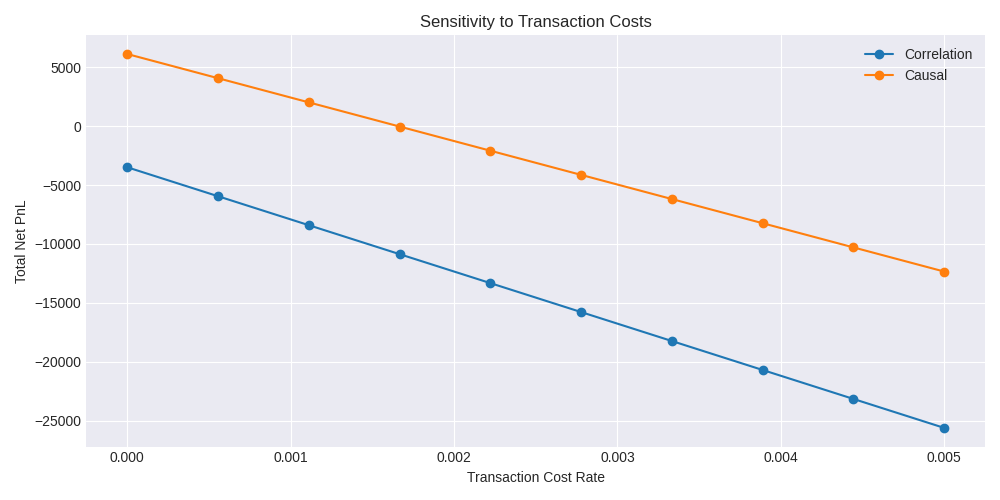
\includegraphics[width=\textwidth,height=0.55\textheight,keepaspectratio]{viz4_tc_sensitivity.png}
            \vspace{0.1cm}
            \scriptsize \\ \textbf{Insight 4}: Causal approach remains profitable up to $\sim30$ bps/trade. Correlation is unviable across the entire cost spectrum.
        \end{column}
        \begin{column}{0.5\textwidth}
            \centering
            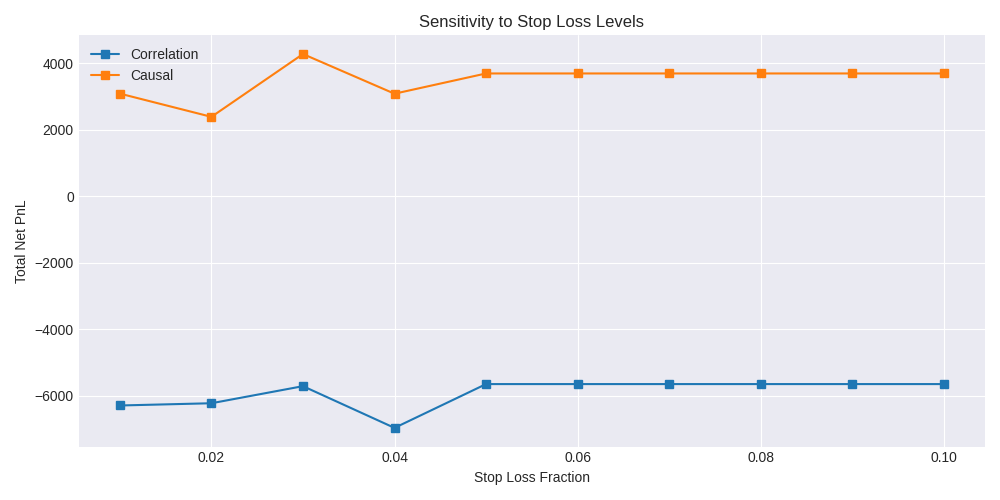
\includegraphics[width=\textwidth,height=0.55\textheight,keepaspectratio]{viz5_sl_sensitivity.png}
            \vspace{0.1cm}
            \scriptsize \\ \textbf{Insight 5}: Optimal stop-loss is $\sim5\%$. Tighter stops ($<3\%$) choke mean-reversion. Wider stops for correlation just increase terminal losses.
        \end{column}
    \end{columns}
\end{frame}

\begin{frame}{Holding Period Constraints \& Half-Life}
    \begin{columns}
        \begin{column}{0.5\textwidth}
            \centering
            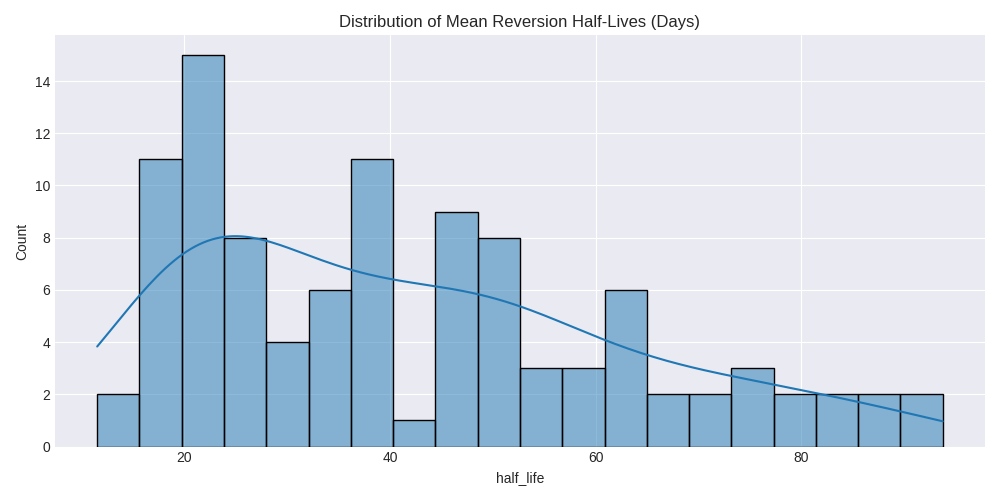
\includegraphics[width=\textwidth,height=0.55\textheight,keepaspectratio]{viz6_halflife.png}
            \vspace{0.1cm}
            \scriptsize \\ \textbf{Insight 6}: Most cointegrated pairs have a half-life of 10-40 days. This mathematically justifies a 30-day max holding constraint.
        \end{column}
        \begin{column}{0.5\textwidth}
            \centering
            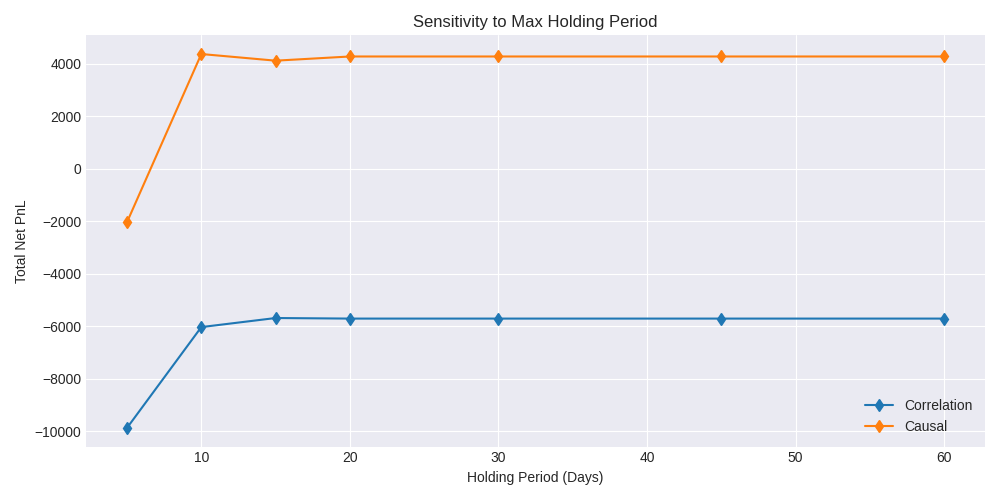
\includegraphics[width=\textwidth,height=0.55\textheight,keepaspectratio]{viz9_hp_sensitivity.png}
            \vspace{0.1cm}
            \scriptsize \\ \textbf{Insight 9}: Returns maximize around 30 days. Shorter limits cut mean-reversion early; longer limits introduce uncompensated drift risk.
        \end{column}
    \end{columns}
\end{frame}

\begin{frame}{Stability and Risk Invariants}
    \begin{columns}
        \begin{column}{0.5\textwidth}
            \centering
            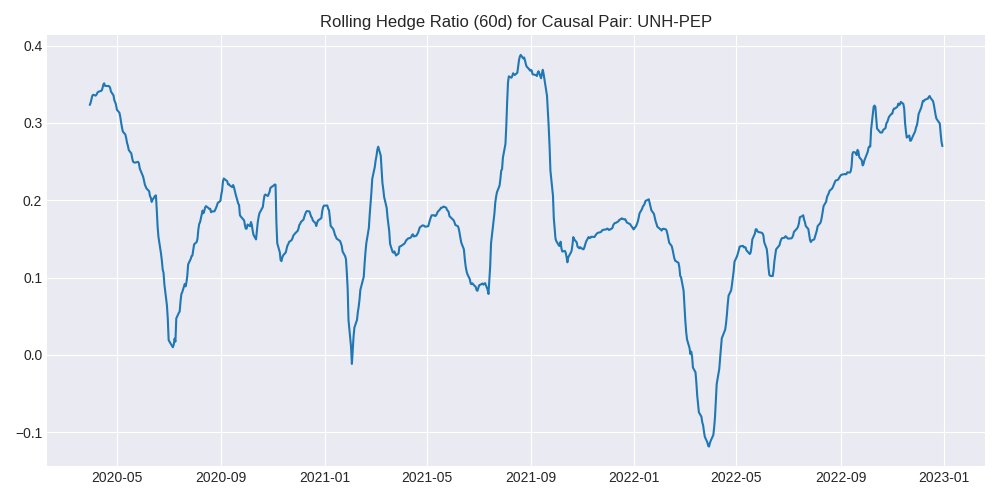
\includegraphics[width=\textwidth,height=0.55\textheight,keepaspectratio]{viz8_rolling_hr.png}
            \vspace{0.1cm}
            \scriptsize \\ \textbf{Insight 8}: 60-day rolling Hedge Ratio ($\beta$) for causal pairs exhibits bounded, mean-reverting stationarity without structural breaks.
        \end{column}
        \begin{column}{0.5\textwidth}
            \centering
            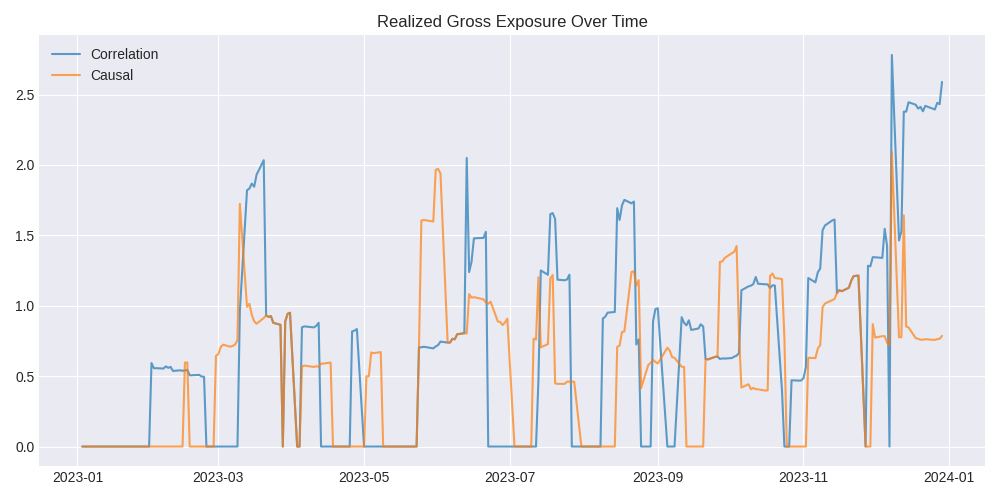
\includegraphics[width=\textwidth,height=0.55\textheight,keepaspectratio]{viz10_exposure.png}
            \vspace{0.1cm}
            \scriptsize \\ \textbf{Insight 10}: Realized gross exposure strictly obeys the 2.0 maximum ceiling, proving the algorithm's capital bound invariants.
        \end{column}
    \end{columns}
\end{frame}

\section{Future Optimization \& Conclusion}
\begin{frame}{Future Extensions}
    \begin{itemize}
        \item \textbf{Maximum Likelihood Estimation (MLE)}: Derive exact discrete-time OU parameters for precise analytical half-life calculation and dynamic thresholding.
        \vspace{0.2cm}
        \item \textbf{Kelly Criterion Sizing}: Implement Fractional Kelly position sizing ($f^* = \frac{\mu_{\text{excess}}}{\sigma_{\text{portfolio}}^2}$) to mathematically maximize the compound growth rate.
        \vspace{0.2cm}
        \item \textbf{Non-linear Transaction Costs}: Incorporate the Almgren-Chriss market impact model (slippage proportional to $\sqrt{V/\text{ADV}}$) for scaling AUM capacity.
    \end{itemize}
\end{frame}

\begin{frame}{Conclusion}
    \begin{itemize}
        \item Simplistic correlation screens routinely fail out-of-sample due to their vulnerability to spurious, historically coincident trends.
        \vspace{0.2cm}
        \item Integrating rigorous causal inference (\textbf{Granger causality}) acts as a powerful structural filter, isolating pairs that possess a genuine information-driven link.
        \vspace{0.2cm}
        \item Our \textbf{Causal Pairs} framework successfully maintained cointegration out-of-sample, preserving capital through drawdowns and generating a positive Sharpe Ratio (0.516) under strict institutional-grade risk limits.
    \end{itemize}
\end{frame}

\begin{frame}[plain, c]
    \begin{center}
        \Huge \textbf{Thank You!} \\
        \vspace{1cm}
        \large \textit{Questions?}
    \end{center}
\end{frame}

\end{document}
